\section{Pregunta N$^{\circ}$9\qquad León Alonzo Terrones Caccha}

\begin{frame}
    \begin{enumerate}\setcounter{enumi}{8}
        \item

              Determine los valores de $n$ y $h$ que se requiere para
              aproximar
              \begin{math}
                  \displaystyle
                  \int\limits_{0}^{4}
                  \dfrac{\dl x}{x+4}
              \end{math}
              con una exactitud de $10^{-5}$ y calcule la
              aproximación aplicando

              \begin{itemize}
                  \item

                        la regla compuesta del trapecio,

                  \item

                        la regla compuesta de Simpson,

                  \item

                        la regla compuesta del punto medio.
              \end{itemize}
    \end{enumerate}

    \begin{solution}
        Sean $a=0$, $b=4$, $h=\dfrac{b-a}{n}$, $x\in\left[a,b\right]$
        y
        \begin{math}
            f\left(x\right)=
            \dfrac{1}{x+4}
        \end{math}.
        Sus primeras cuatro derivadas son

        \begin{align*}
            f^{\left(1\right)}\left(x\right) &
            =\dfrac{-1}{{\left(x+4\right)}^{2}}. \\
            f^{\left(2\right)}\left(x\right) &
            =\dfrac{2}{{\left(x+4\right)}^{3}}.  \\
            f^{\left(3\right)}\left(x\right) &
            =\dfrac{-6}{{\left(x+4\right)}^{4}}. \\
            f^{\left(4\right)}\left(x\right) &
            =\dfrac{24}{{\left(x+4\right)}^{5}}.
        \end{align*}
    \end{solution}
\end{frame}

\begin{frame}
    %\frametitle{Reglas de cuadratura}
    \begin{solution}
        \begin{itemize}
            \item

                  Regla compuesta de Simpson.

                  Como
                  \begin{math}
                      f^{\left(4\right)}
                      \left(x\right)\leq
                      \dfrac{24}{{\left(x+4\right)}^{5}}
                  \end{math},
                  entonces

                  \begin{align*}
                      \left|E\left(n\right)\right| & =
                      \dfrac{{\left(b-a\right)}^{5}}{180n^{4}}
                      f^{\left(4\right)}
                      \left(\xi\right)                    \\
                                                   & \leq
                      \dfrac{2}{15n^{4}}.
                      \shortintertext{Para un error menor que $10^{-5}$,}
                      n^{4}                        & >
                      \dfrac{2}{15}10^{5}.                \\
                      n                            & >
                      10.74.
                  \end{align*}

            \item

                  Regla compuesta del trapecio.

                  \begin{align*}
                      \left|E\left(n\right)\right| & =
                      \dfrac{\left(b-a\right)^{3}}{12n^{4}}
                      f^{\left(4\right)}\left(\xi\right)      \\
                                                   & \leq
                      \dfrac{1}{6n^{2}}.
                      \shortintertext{Para un error menor que $10^{-5}$,}
                      n^{2}                        & >
                      \dfrac{1}{6}10^{5}.                     \\
                      n                            & >129.09.
                  \end{align*}
        \end{itemize}
    \end{solution}
\end{frame}

\begin{frame}
    \begin{solution}
        \begin{itemize}
            \item

                  Regla compuesta del punto medio.

                  Como
                  \begin{math}
                      f^{\left(2\right)}
                      \left(x\right)\leq
                      \dfrac{2}{{\left(x+4\right)}^{3}}
                  \end{math},
                  entonces

                  \begin{align*}
                      \left|E\left(n\right)\right| & =
                      \dfrac{{\left(b-a\right)}^{3}}{6{\left(n+2\right)}^{2}}
                      f^{\left(2\right)}
                      \left(\xi\right)                    \\
                                                   & \leq
                      \dfrac{1}{3n^{2}}.
                      \shortintertext{Para un error menor que $10^{-5}$,}
                      {\left(n+2\right)}^{2}       & >
                      \dfrac{1}{3}10^{5}.                 \\
                      n                            & >
                      180.57.
                  \end{align*}
        \end{itemize}
    \end{solution}
\end{frame}

\begin{frame}{Resultados-Python}
    \begin{figure}
        \centering
        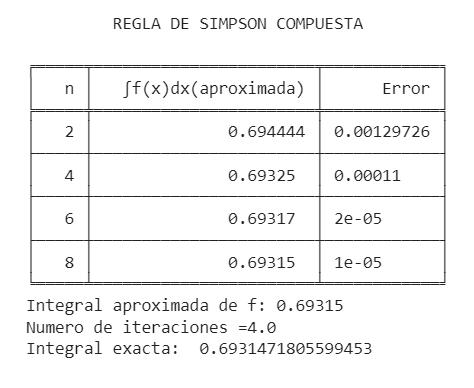
\includegraphics[width=12cm]{p9-simpson.png}
        %\caption{Caption}
        \label{fig:enter-label}
    \end{figure}
\end{frame}

\begin{frame}{Resultados-Python}
    \begin{figure}
        \centering
        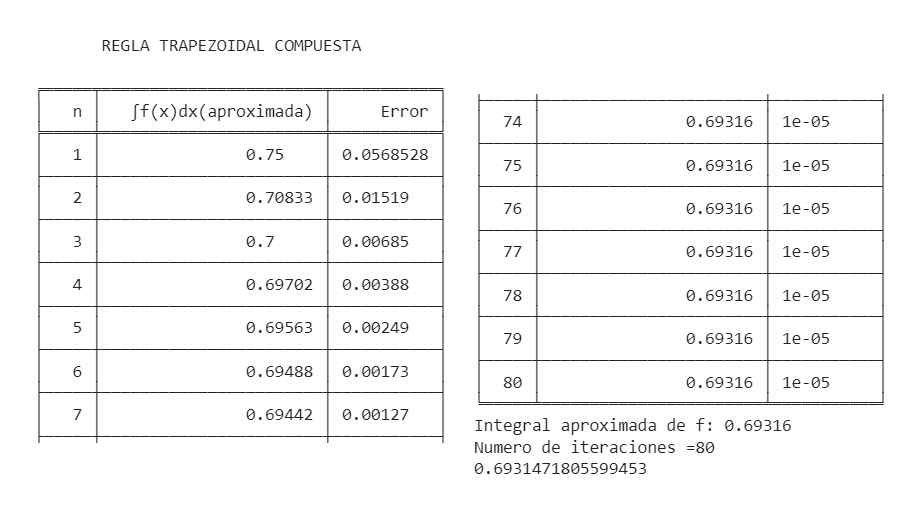
\includegraphics[width=12cm]{p9-trap.png}
        %\caption{Caption}
        \label{fig:enter-label}
    \end{figure}
\end{frame}

\begin{frame}{Resultados-Python-}
    \begin{figure}
        \centering
        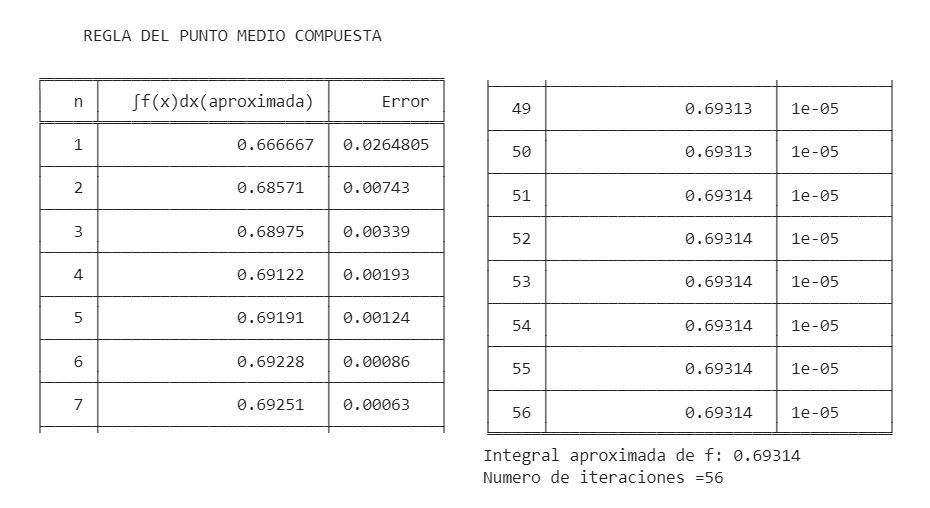
\includegraphics[width=12cm]{p9-pmedio.png}
        %\caption{Caption}
        \label{fig:enter-label}
    \end{figure}
\end{frame}
